

Flow graphs are an abstraction used to represent elements (\eg digital data, goods, electric current) that travel through a network of nodes (\eg computers, physical locations, circuit parts). Flow graphs are often used in the modelling of logistics problems. Weights associated with the edges represent either the size of the load that is transmitted from the source to the destination node, or the frequency of transmission of a token between these nodes. The nodes of a flow graph may have associated weights that can represent, for instance, the capacity of the node, or the cost of storing payload at the node, or the delay of processing a token at that node. If additional data, in the form of attributes and their values, are associated with the nodes, we have attributed flow graphs. An attributed flow graph (AFG) is a single-entry/single-exit graph with a \emph{source node} that has no incoming edges and a \emph{sink node} with no outgoing edges. The flow starts in the source node and is directed to the sink node. All other nodes in the AFG, if they exist, must have at least one incoming and one outgoing edge. An example of an AFG is shown in Figure~\ref{fig:AFG}.

\begin{figure}[htp]
\centering
\begin{tabular}{cc}
 %   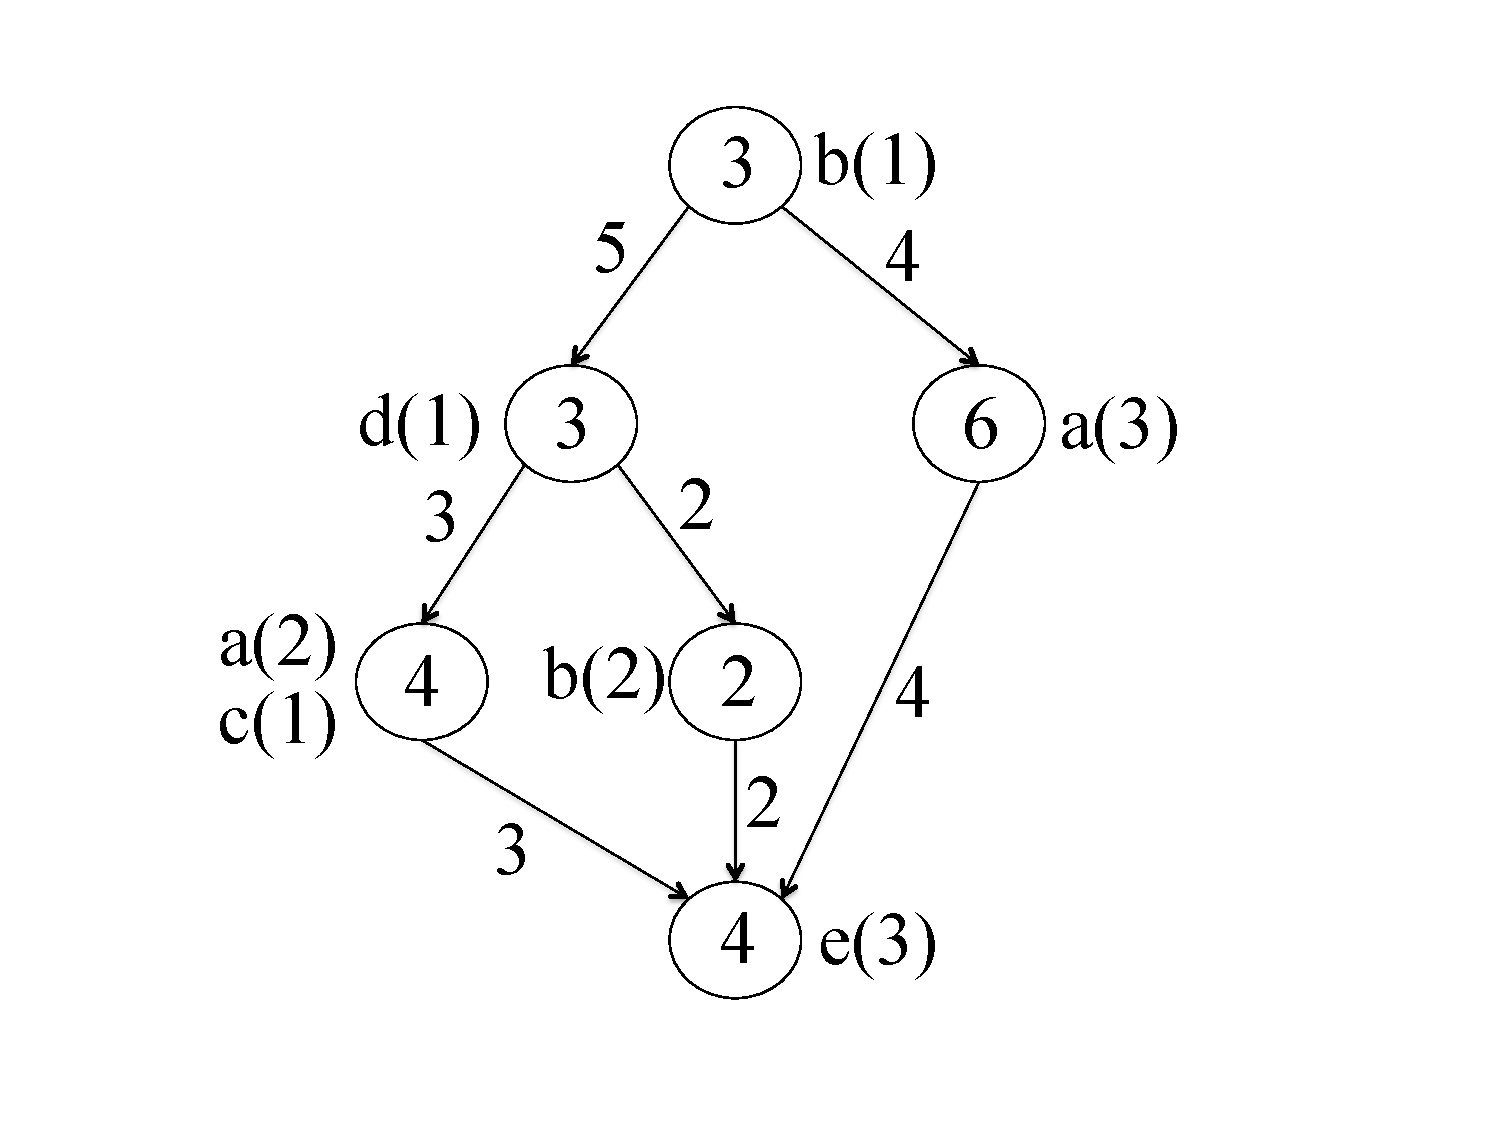
\includegraphics[scale=0.2]{figures/attributed_flow_graph2.eps}
  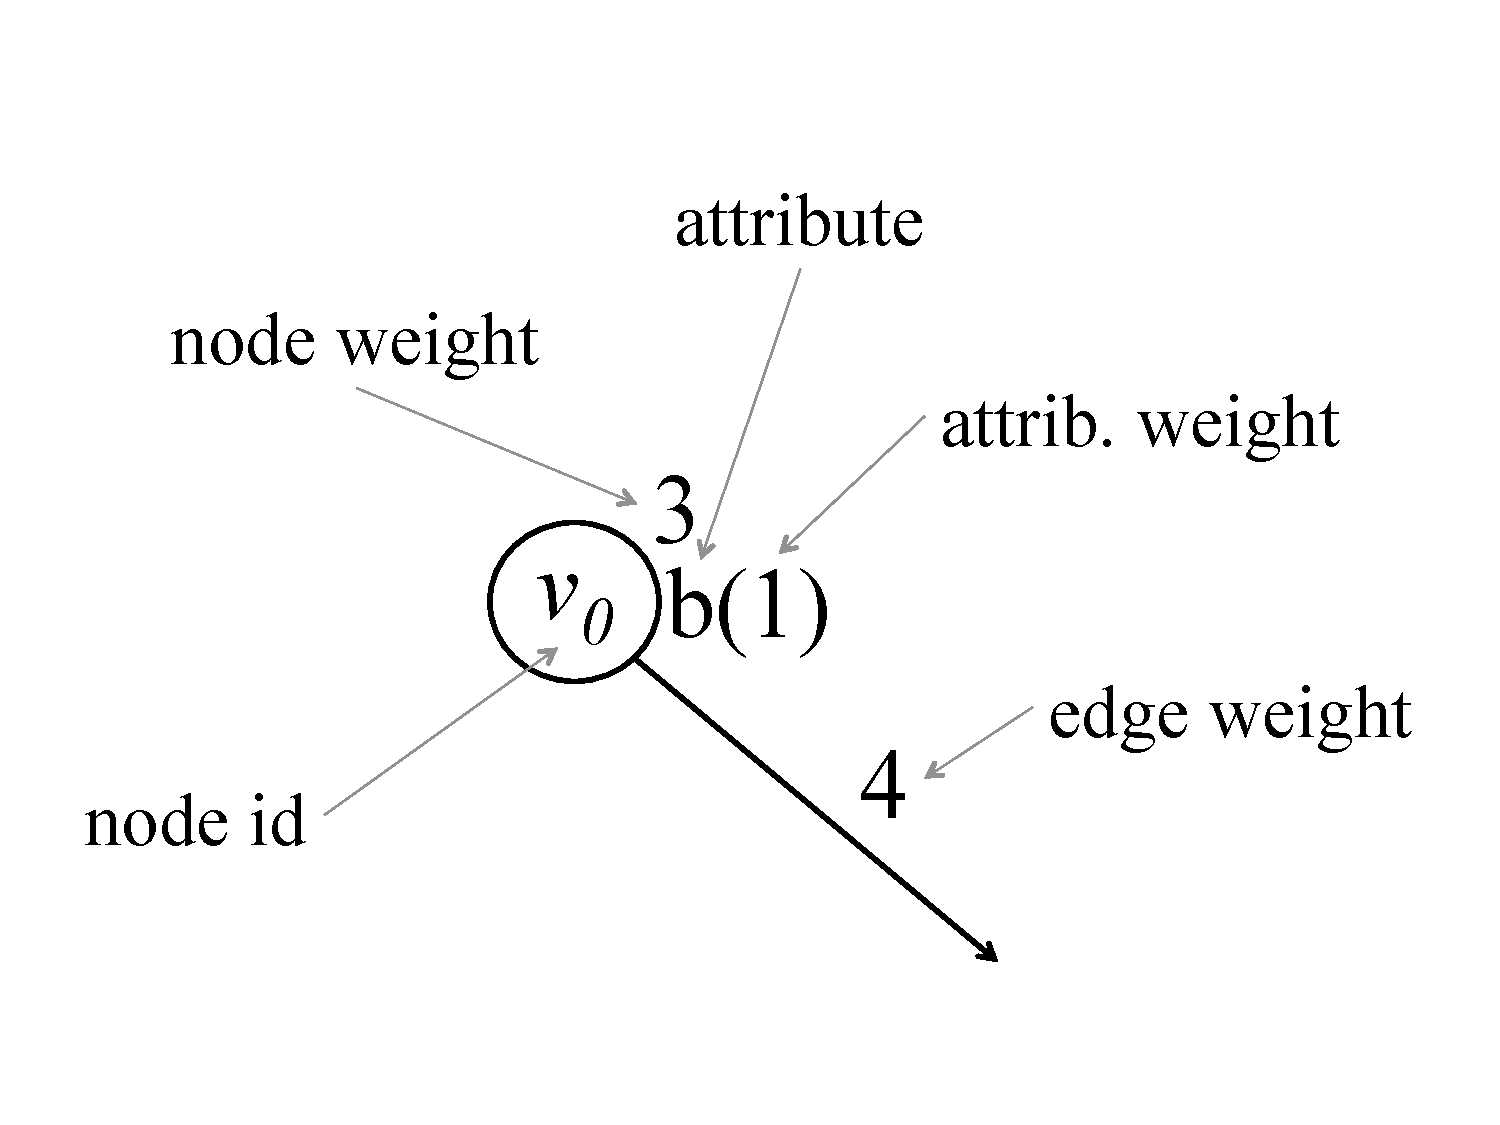
\includegraphics[scale=0.18]{figures/attributed_flow_graph_descpr.pdf} &
  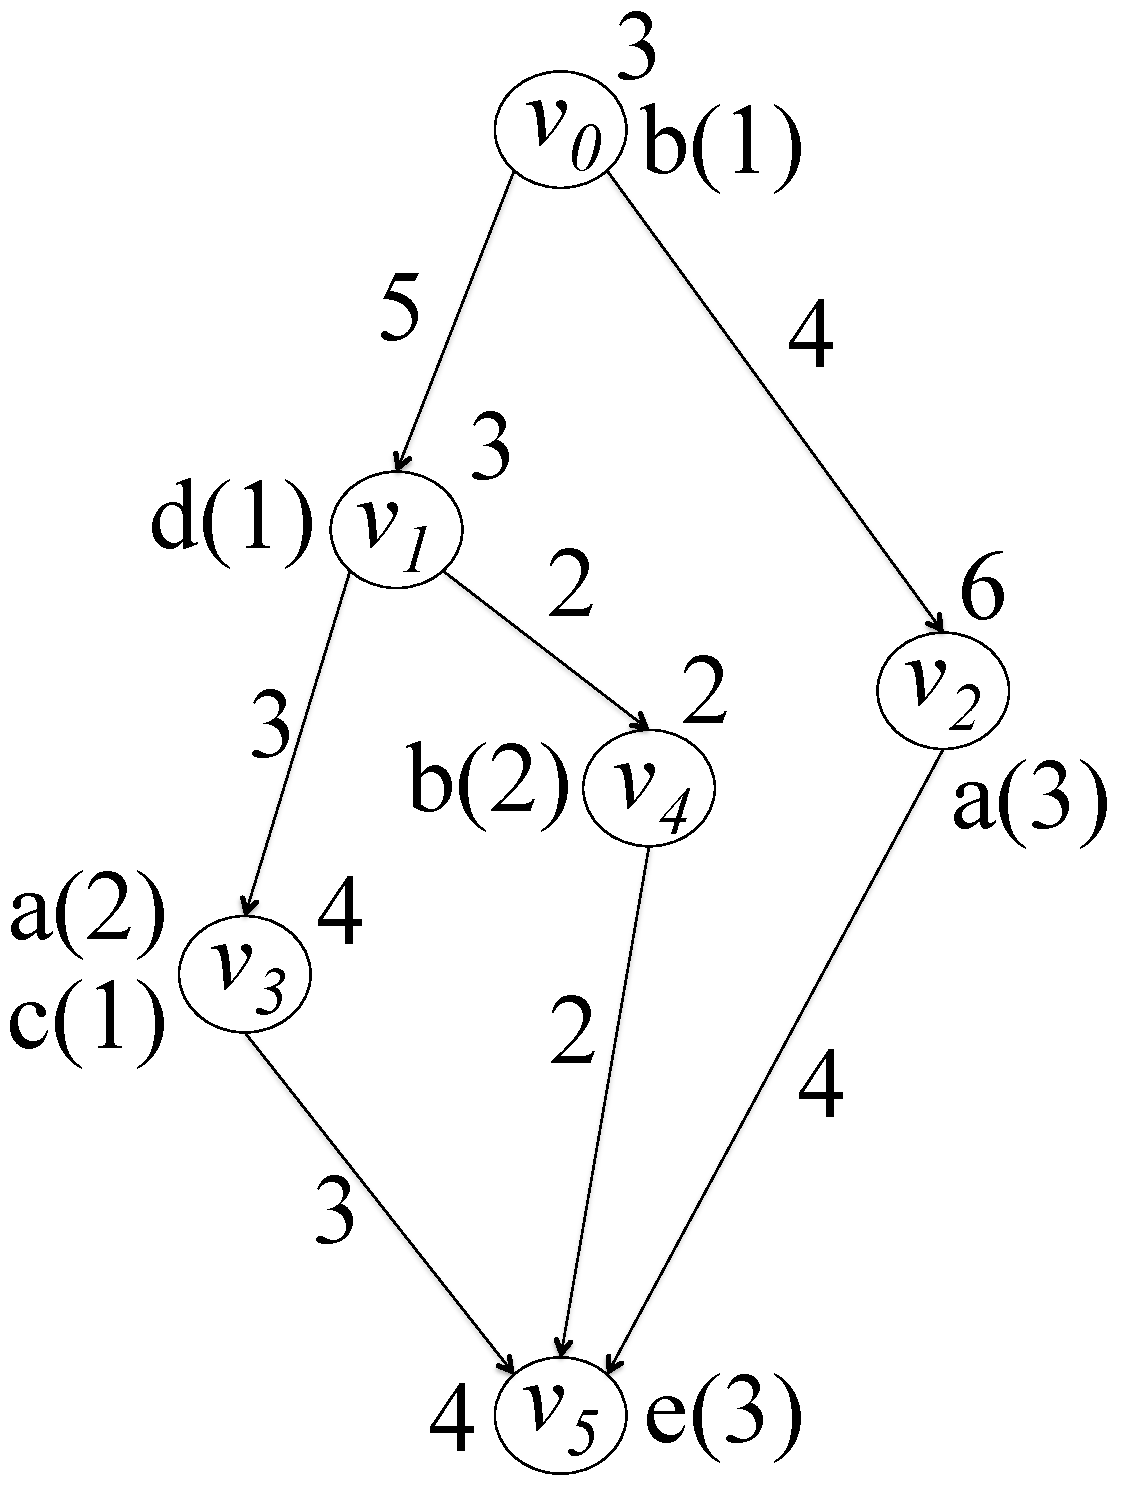
\includegraphics[scale=0.18]{figures/attributed_flow_graph3.pdf}\\
  (a) Elements of an AFG & (b) Example
\end{tabular}
    \caption{Example of attributed flow graph.}
    \label{fig:AFG}  
\end{figure}

The presence of weights associated with edges, nodes and attributes allows AFGs --- either a single AFG or a set of AFGs --- to create a rich description of dynamic applications. It might be best to illustrate an AFG thtrough an example that models logistics. Figure~\ref{fig:Airport} shows a snapshot of the transportation by air of goods between cities. In this illustrative example, an AFG models the volume of sea food, medicine, and flowers processed through the cargo terminals of several airports. Airports are represented as nodes, the type of goods processed at an airport as attributes of each node, the volume of each type of good handled in an airport as attribute weights, the storage capacity at each airport as node weights, and the volume capacity of the flights transporting goods between cities are represented as weighted directed edges. With similar data for multiple transportation companies, an analyst may use a set of AFGs to model a transportation network with each AFG, for instance, corresponding to a single company.  

\begin{figure}[h!]
\centering
%    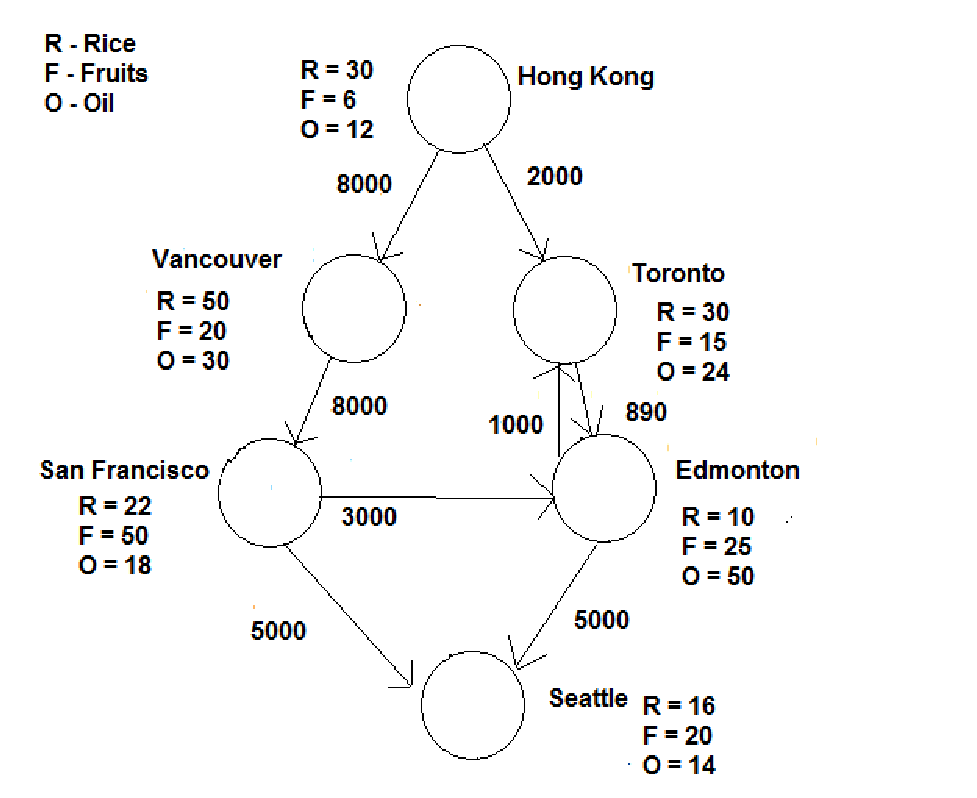
\includegraphics[scale=0.3]{figures/attributed_flow_graph_airport.eps}
  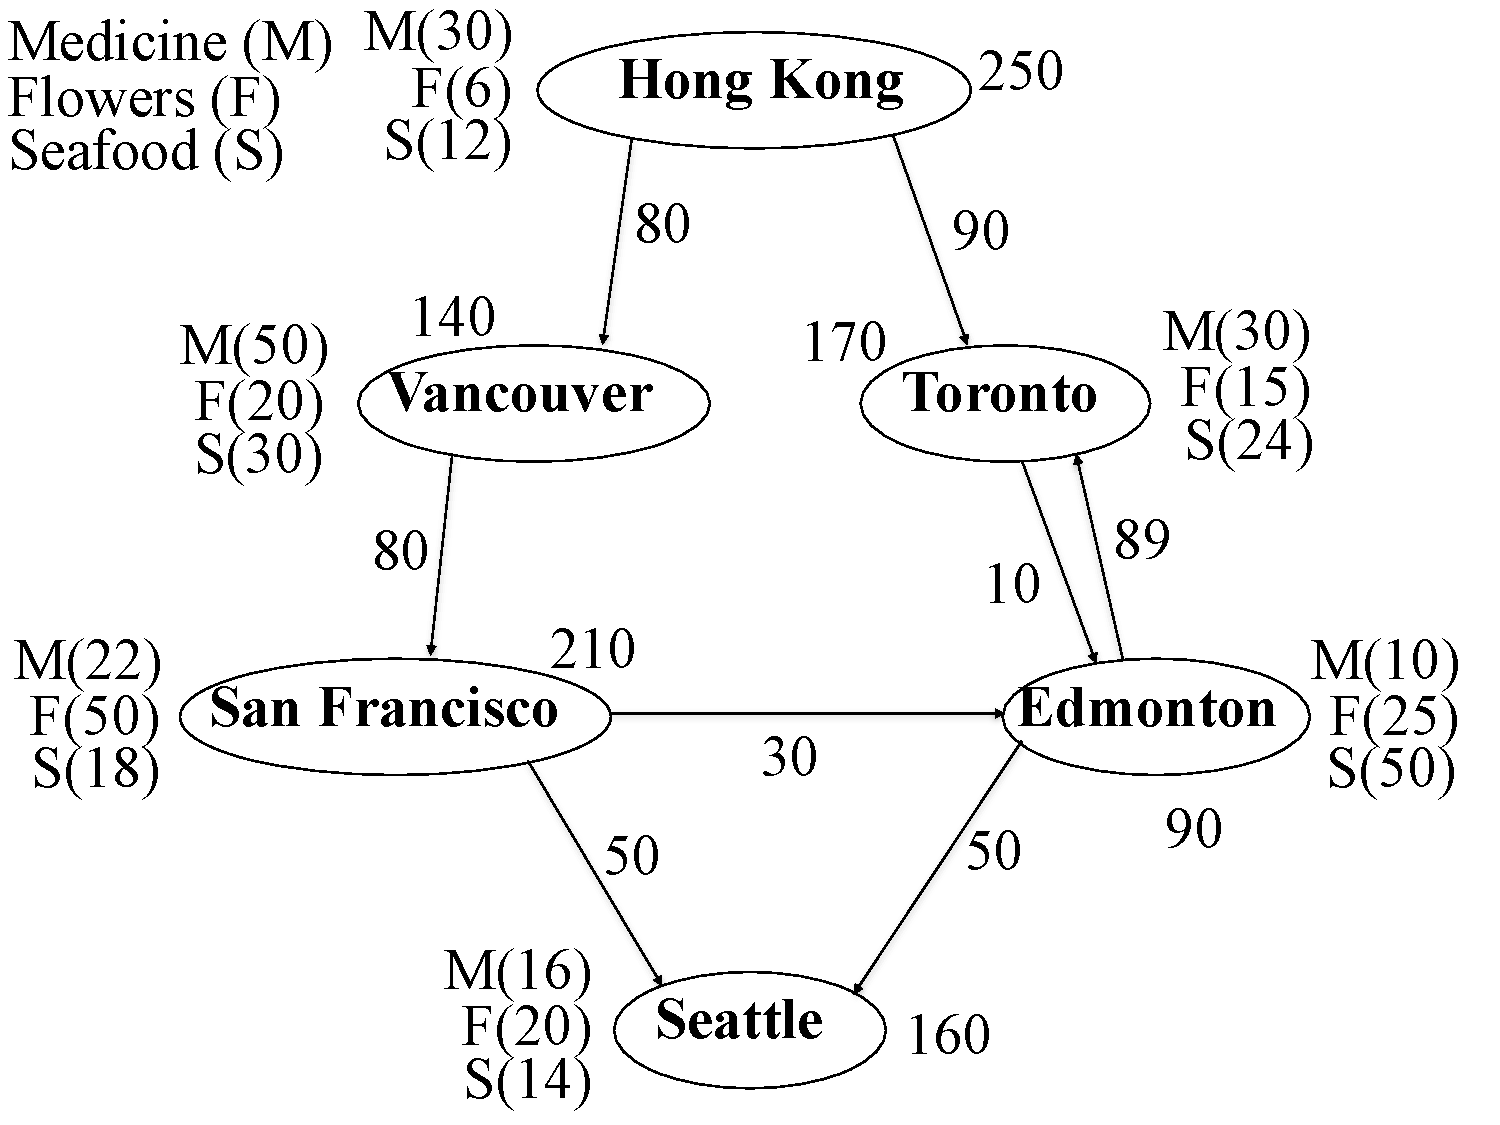
\includegraphics[scale=0.2]{figures/attributed_flow_graph_airport2.pdf}
    \caption{AFG representing transportation of goods between airports.}
    \label{fig:Airport}  
\end{figure}

In many applications modelled by AFGs, complex structural sub-graph patterns may be prevalent. These sub-graphs are often unknown and non-trivial to detect, but they may represent important characteristics of the application. Given the richness of the model, the notion of ``prevalence'' or ``support'' of such patterns, as a measure of interestingness or importance to analysts, is often difficult to capture by simply counting the number of occurrences of the pattern in the AFG. Instead, when modelling an application with AFGs the interesting and useful patterns that an analyst wants to detect are also characterized by node attributes and a notion of support that may include node weights, attribute weights and edge weights. 

\begin{figure}[h!]
\centering
%    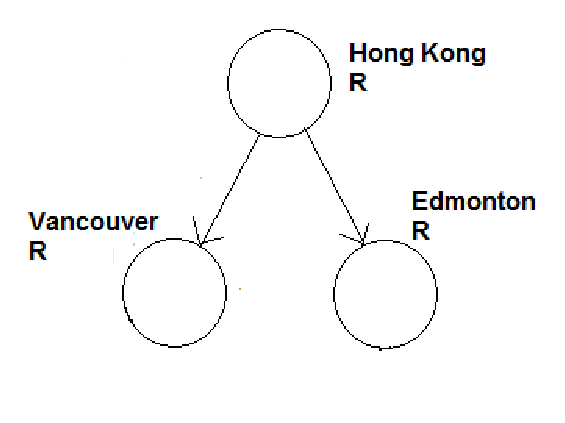
\includegraphics[scale=0.1]{figures/pattern_airport.eps}
   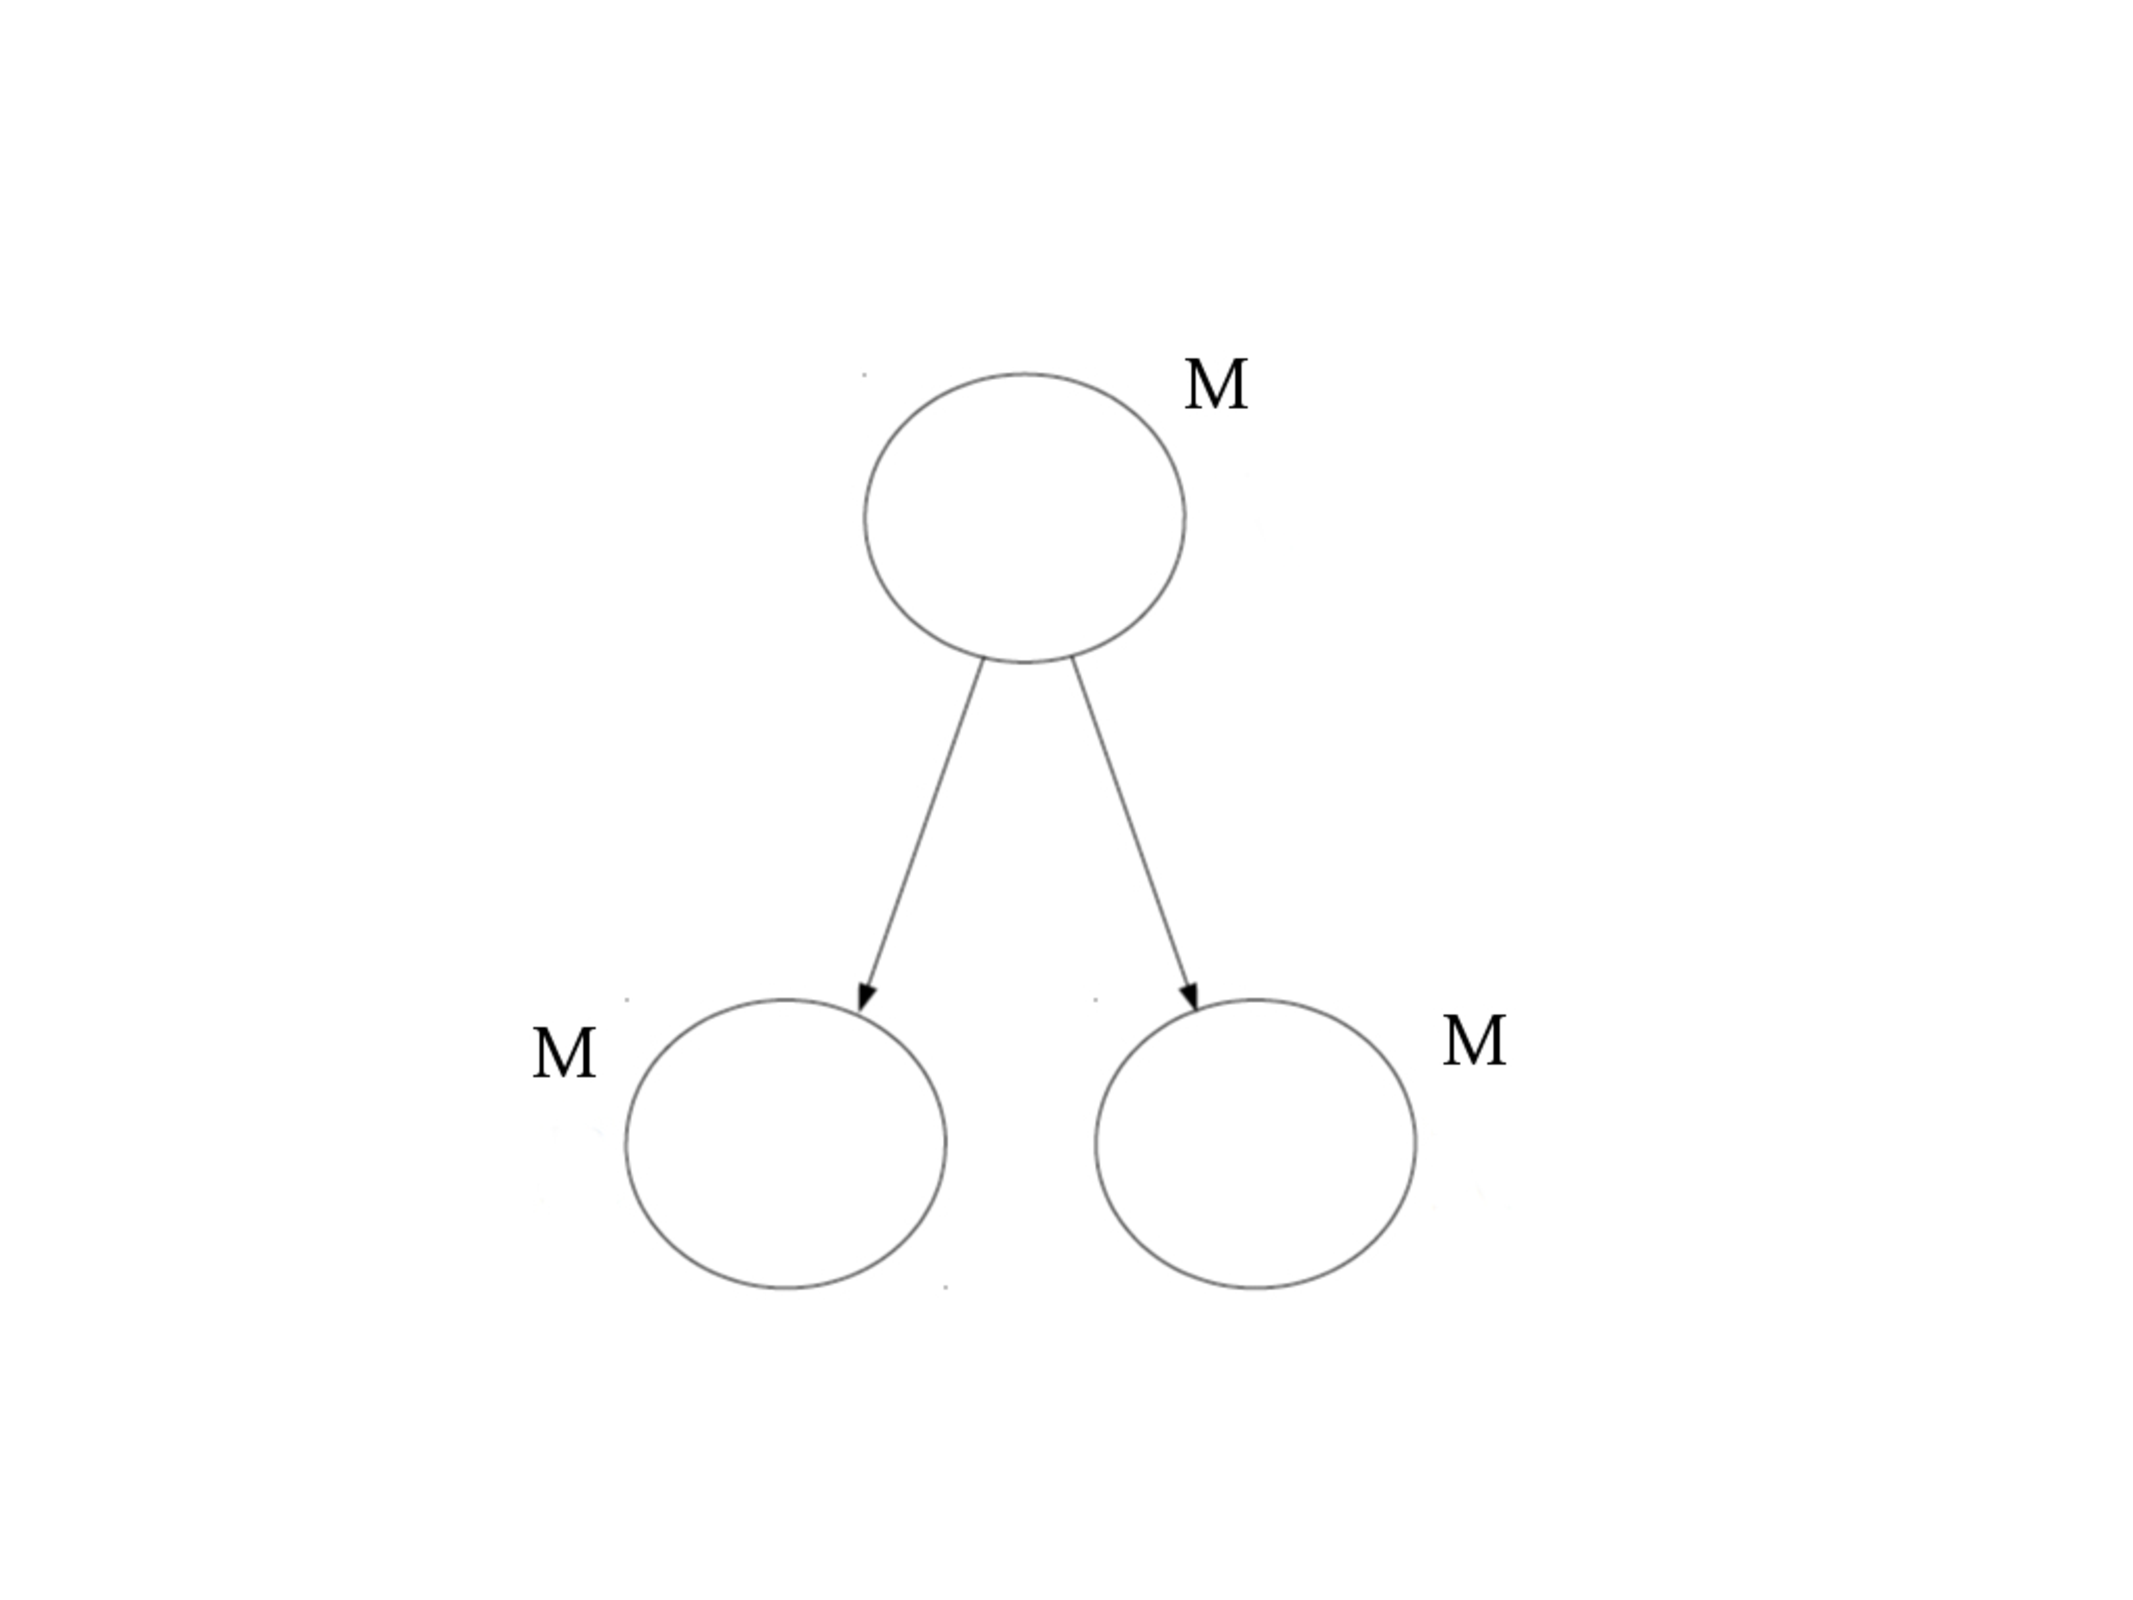
\includegraphics[scale=0.1]{figures/figure3.pdf}
    \caption{Pattern in the goods distribution example.}
    \label{fig:Pattern}  
\end{figure}

Different applications may benefit from using other definitions of a support metric that takes more than the frequency of pattern occurrences into account. Section~\ref{sec:CaseStudies} discusses an application of AFGs in compiler optimization and software profiling. Although the remainder of this paper will not discuss logistics-based problems, the example in Figure~\ref{fig:Airport} seeks to underscore that AFGs and methods to discover supported patterns in AFGs are broadly applicable. However, such a method that takes the full structural information present in AFGs into account while searching for patterns does not exist.

Existing graph-mining algorithms are all severely limited in their applicability to AFGs. None of them is able to find general sub-graph patterns in AFGs that take into account multiple node attributes as well as weights in nodes and edges. A number of algorithms proposed in the literature perform sub-graph mining only on undirected and unweighted graphs, with no attributes~\cite{gSpan}~\cite{Gaston}~\cite{FFSM}~\cite{FSP}~\cite{AGM}. Such algorithms mine datasets of graphs for \emph{frequent sub-graphs}, which are patterns that occur more than a certain number of times in the dataset. 

The only work on mining patterns in AFGs is the FlowGSP algorithm proposed by \emph{Jocksch~\etal}~\cite{FlowGSP}. However, FlowGSP can only find sub-path patterns, while the algorithm described in this work finds all the patterns that FlowGSP does and additional patterns that encompass multiple sub-paths in the dataset.  

This paper presents AFGMiner, the first algorithm, to the best of our knowledge, to address the problem of mining AFGs for general sub-graph patterns. AFGMiner takes as input a set of AFGs and a support measure $MinSup$ that may be formulated by taking into account the attribute weights, node weights and edge weights of the occurrences of patterns. AFGMiner returns all patterns $P$, called \emph{heavyweight patterns}, whose support $MinSup(P)$ is higher than a threshold. This threshold is user-specified as commonly assumed in pattern-mining approaches.
The main contributions of this paper are as follows: 

\begin{enumerate}
\item Definition of the Attributed-Flow-Graph Mining problem to find Heavyweight Patterns.

\item Development of different versions of AFGMiner, an algorithm that mines for heavyweight patterns in attributed flow graphs, including a parallel version with a work-distribution heuristic to maintain workload balance between multiple threads.

\item Development of HEPMiner, a tool that automates the analysis of hardware-instrumented profiles. HEPMiner allows compiler developers to mine for heavyweight patterns that represent particular \emph{execution patterns}. Discovered patterns indicate potential, non-obvious, opportunities for compiler and architecture-design improvements.

\item Complexity and scalability analysis of AFGMiner, comparison against the FlowGSP algorithm and qualitative analysis of patterns found by HEPMiner when applied to the DayTrader benchmark running on IBM's WebSphere Application Server~\cite{WAS}.
\end{enumerate} 




